%\begin{frame}{Overview}
%    % \emphSlide{IntraJ} is an application of \emphSlide{IntraCFG}
%    \hspace*{-0.7cm}%
%    \only<1>{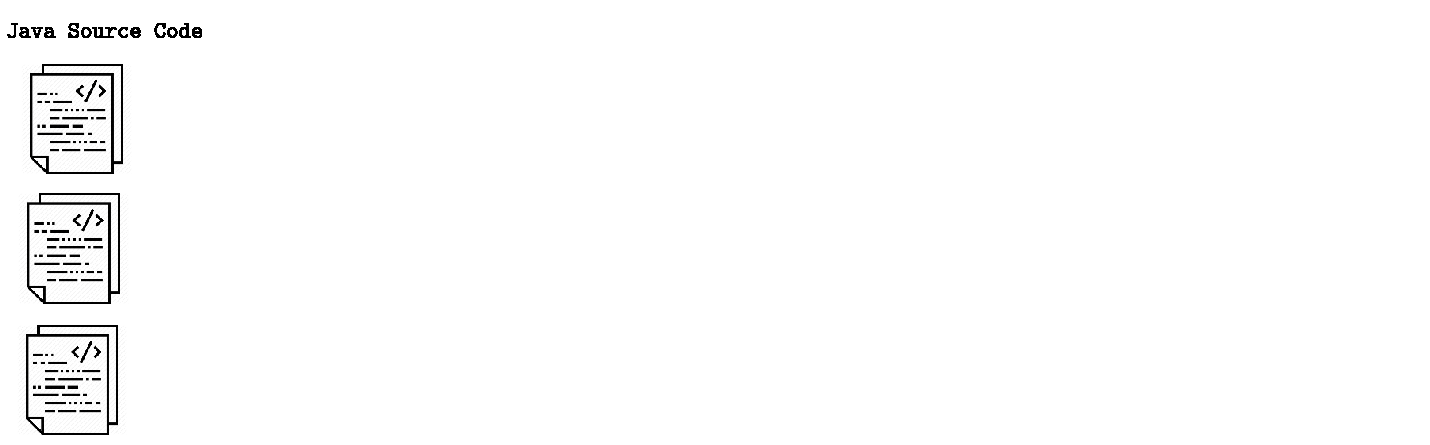
\includegraphics[scale=0.5]{img/intraj1.pdf}}%
%    \only<2>{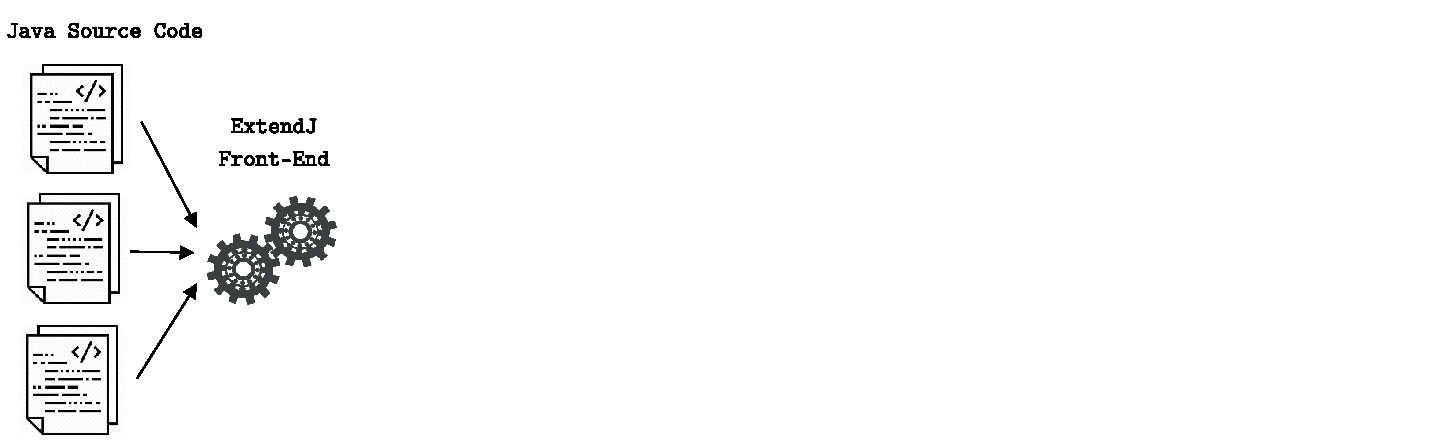
\includegraphics[scale=0.5]{img/intraj2.pdf}}%
%    \only<3>{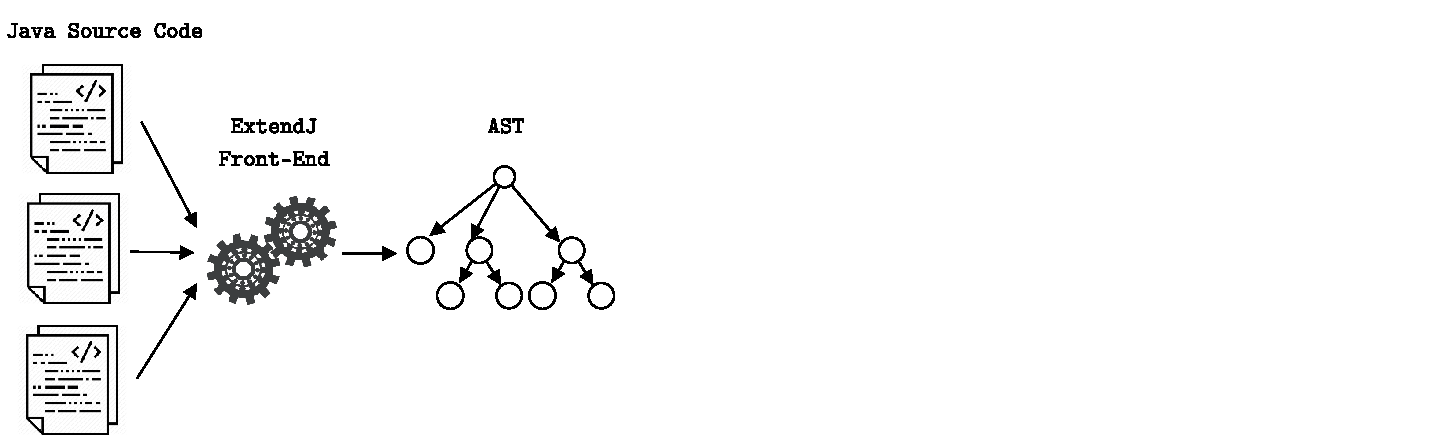
\includegraphics[scale=0.5]{img/intraj3.pdf}}%
%    \only<4>{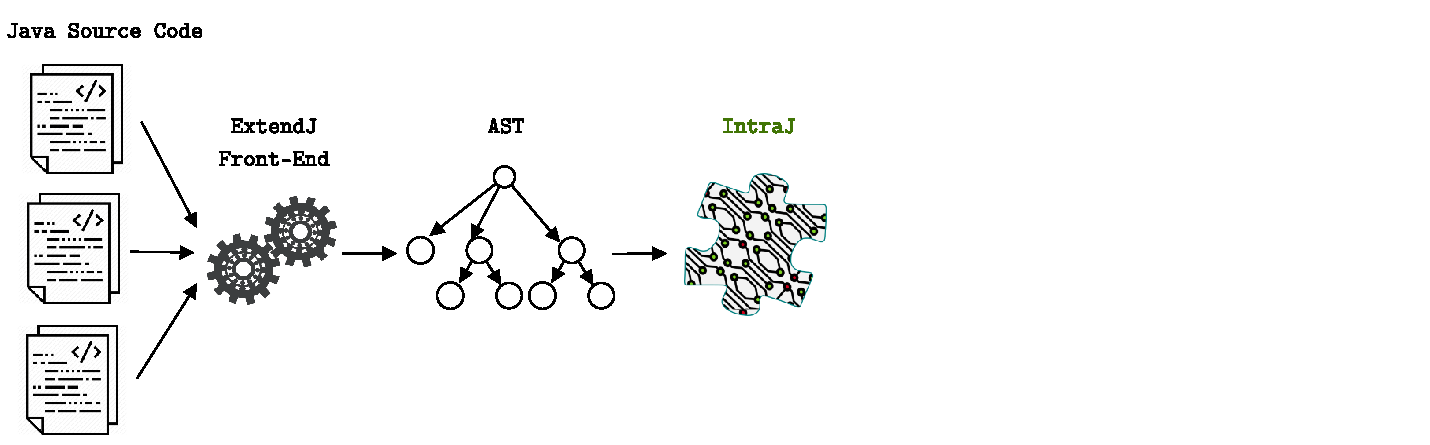
\includegraphics[scale=0.5]{img/intraj4.pdf}}%
%    \only<5>{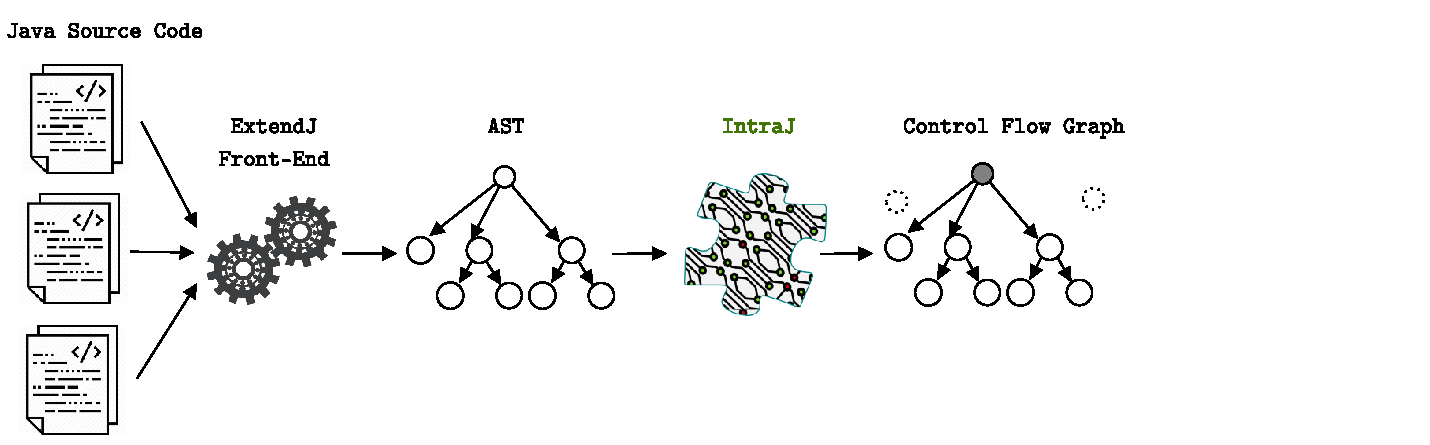
\includegraphics[scale=0.5]{img/intraj51.pdf}}%
%    \only<6>{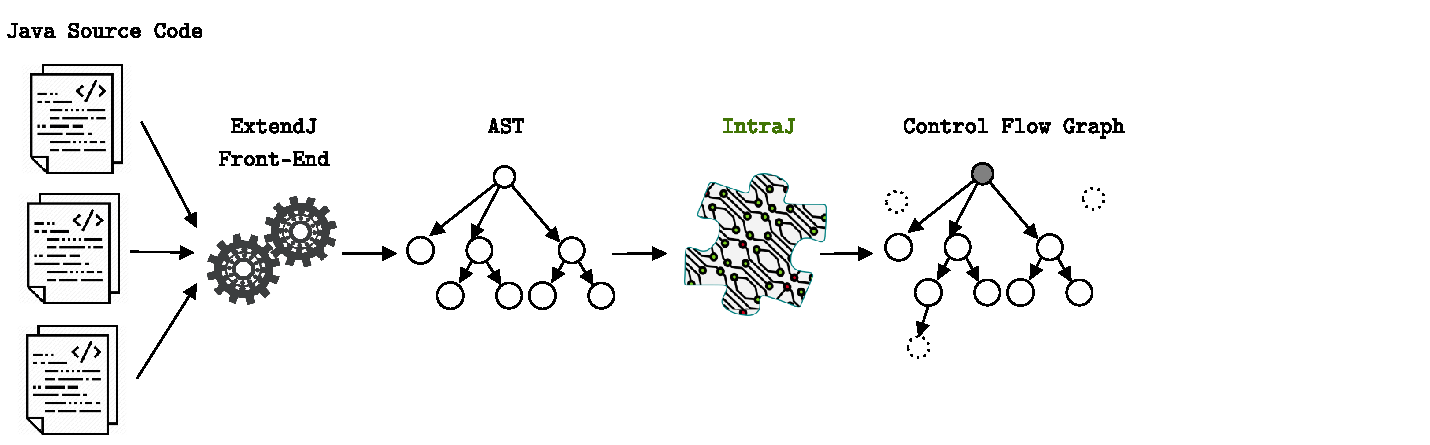
\includegraphics[scale=0.5]{img/intraj52.pdf}}%NTA
%    \only<7>{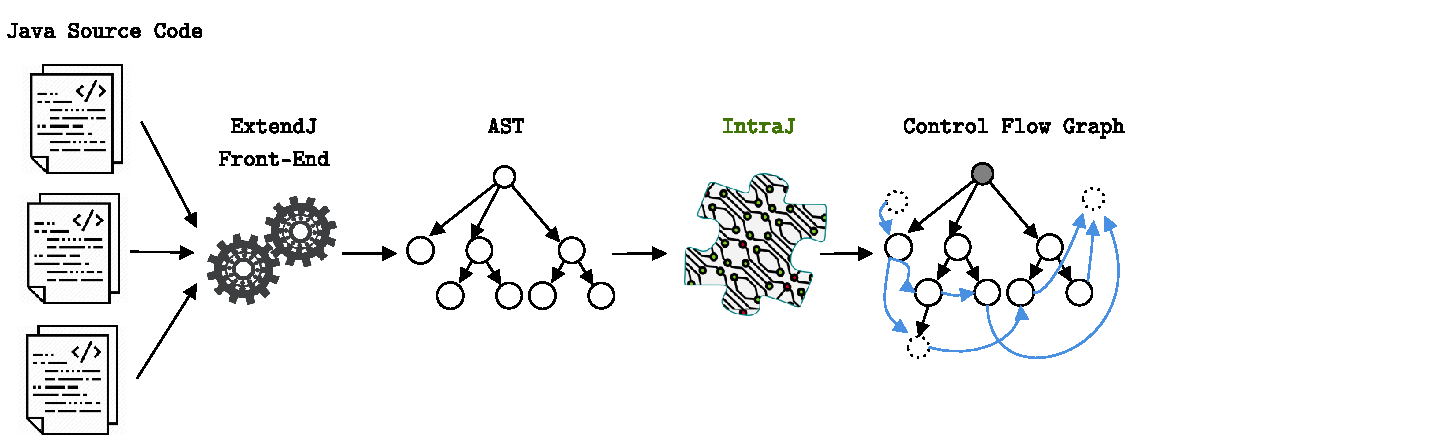
\includegraphics[scale=0.5]{img/intraj53.pdf}}%succ
%    \only<8>{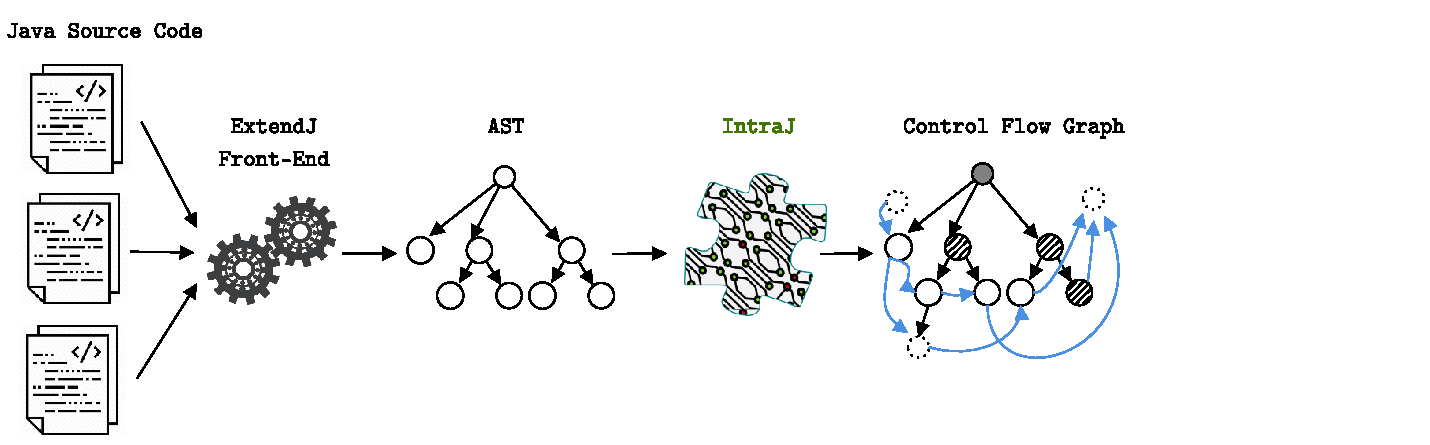
\includegraphics[scale=0.5]{img/intraj54.pdf}}%CFGSupport
%    \only<9>{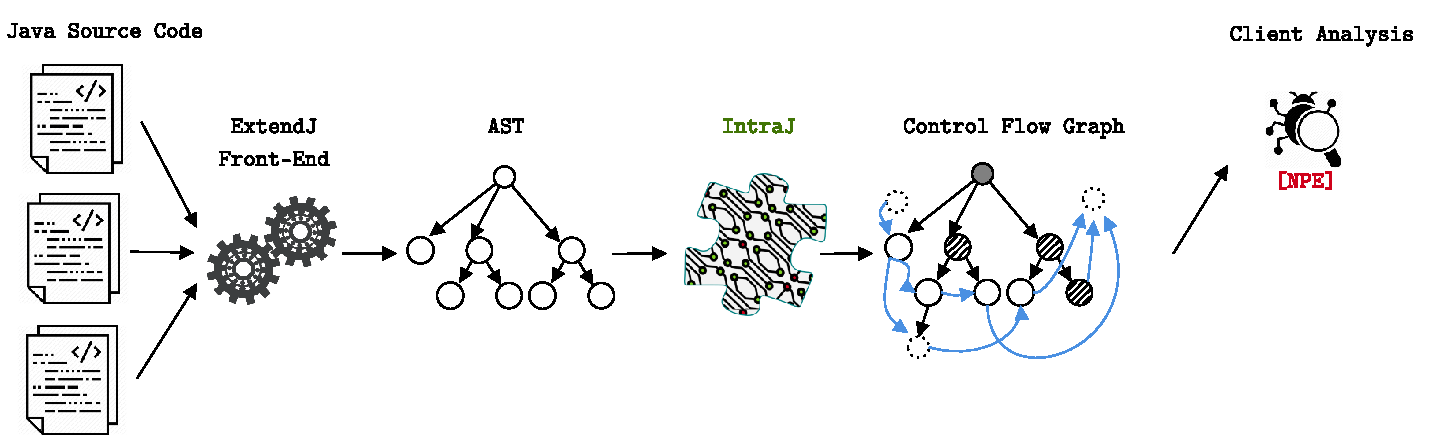
\includegraphics[scale=0.5]{img/intraj6.pdf}}%
%    \only<10>{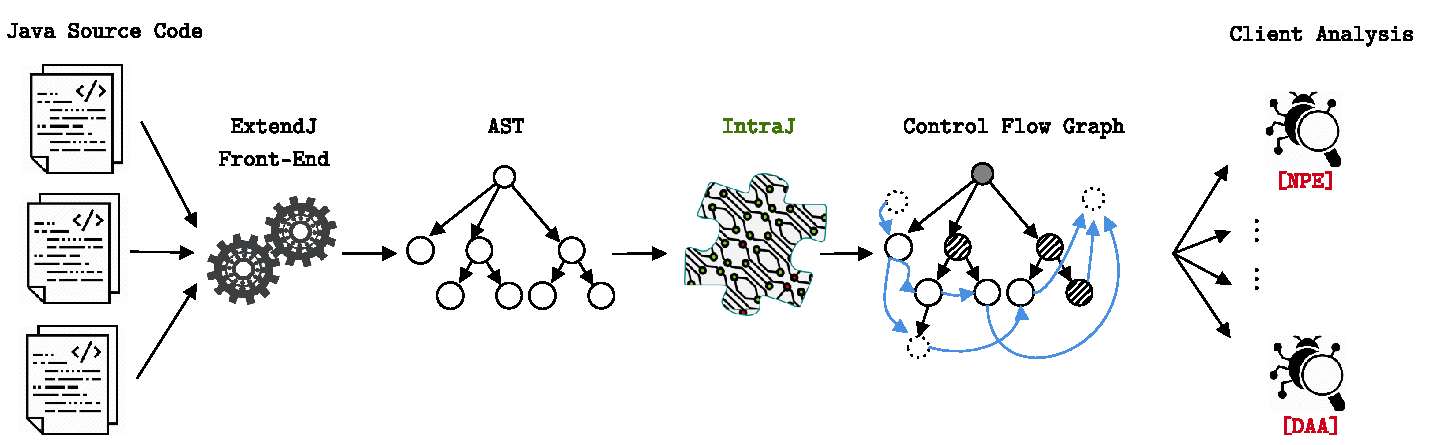
\includegraphics[scale=0.5]{img/intraj7.pdf}}%
%    \begin{multicols}{2}
%        \begin{itemize}
%            \item<2-> \emphSlide{IntraJ} is an extension of \lowEmph{ExtendJ} Java Compiler
%            \item<4-> \emphSlide{IntraJ} superimpose the CFGs on the attributed AST generated by ExtendJ
%            \item<6-> \emphSlide{Precision}: HOAs to reify implicit facts
%            \item<8-> \emphSlide{Minimality}: redundant nodes are excluded
%        \end{itemize}
%    \end{multicols}
%\end{frame}
%
%\begin{frame}{Overview}
%\emphSlide{IntraJ} is an application of the \emphSlide{IntraCFG} framework. We implemented IntraJ as an extension of the \lowEmph{ExtendJ} Java compiler.
%
%Our two main goals were:
%	\begin{itemize}
%		\item Minimality: build concise CFG by excluding AST nodes that do not correspond to any \textit{runtime action}.
%		\item High Precision: the constructed CFGs should capture most program \textit{details}.
%	\end{itemize}
%\end{frame}
%
%

